\ifdefined\XeTeXrevision\else\pdfoutput=1\fi
\documentclass[11pt]{article}
\usepackage[margin=1in]{geometry}
\usepackage{graphicx}
\usepackage{booktabs}
\usepackage{amsmath}
\usepackage{amssymb}
\usepackage{xcolor}
\usepackage{hyperref}
\usepackage{microtype}
\hypersetup{
  colorlinks=true,
  linkcolor=blue!60!black,
  citecolor=blue!60!black,
  urlcolor=blue!60!black,
  pdftitle={Two Regimes of Compressed Conditioning: Basis-Mixture Bridges for Frozen Language Models},
  pdfauthor={Franci Penov},
}
\graphicspath{{figures/}}
\title{Two Regimes of Compressed Conditioning:\\Basis-Mixture Bridges for Frozen Language Models}
\author{Franci Penov \\ kortexa.ai \\ \texttt{francip@kortexa.ai}}
\date{2026-07-03}

\begin{document}
\maketitle

\begin{abstract}
Conditional LoRA bridges condition a frozen language model on an external sensor stream by generating per-input low-rank weight updates, but the generating hypernetwork is dominated by one dense output layer that scales with the adapted model. We reparameterize that output as $k$ coefficients over a learned basis of LoRA directions and characterize the design space on a pretrained 230M-parameter model with capacity-matched controls, task-aligned probes, and weight-space diversity probes. Two regimes emerge. With a small \emph{trained} basis ($k{=}16$; 16$\times$ fewer parameters), the bridge matches the dense hypernetwork's language-modeling gain and its six-way task conditioning, and the diversity--quality tradeoff dissolves: cross-input cosine of generated weights falls from 1.00 to 0.01 with no loss of language-modeling improvement, where the dense bridge pays for every increment. With a large \emph{frozen} basis ($k{=}256$, reconstructible from a random seed), only 181,120 parameters (0.09\% of dense) train, and the bridge reaches the dense model's hard-task conditioning at roughly twice the training steps. At the standard budget that step-for-parameter trade applies to every basis size we tested on the fifty-way task. Mapping frozen-basis conditioning across five widths per task replaces the threshold we first reported with a ramp: conditioning rises monotonically and gradually with $k$, and the two tasks' ramps are offset rather than sharing a boundary. A frozen subspace of 48 directions already carries six-way IMU conditioning while the fifty-way audio probe is still at chance, and audio does not lift until 96. We also report what fails: accelerating basis training destabilizes it; training the basis at large $k$ is mildly harmful; and composing bridges by coefficient averaging inherits the sub-additivity of weight averaging. The obstacle is the merge operation, not the representation.
\end{abstract}

\section{Introduction}
A conditional LoRA bridge \cite{penov2026bridges} maps features from a frozen sensor encoder to per-input Low-Rank Adaptation (LoRA) parameters injected into a frozen language model, giving the model an ambient, token-free awareness of an external signal. The original study established an evaluation discipline (language-modeling metrics cannot certify conditioning; capacity-matched controls and task-aligned probes can) and named its scaling bottleneck: the bridge's final linear layer emits the full flattened LoRA vector, so its parameter count grows with the adapted model. On the 230M-parameter model used here, the dense bridge has 199M parameters against a 774,144-dimensional LoRA vector \cite{penov2026note}.

This paper attacks that bottleneck by construction. The bridge's output layer is replaced by a coefficient head: the hypernetwork emits $k$ coefficients $c$, and the generated weights are $w = c \cdot B$ for a $k \times D$ basis $B$ of LoRA directions. Compression is trivial by construction; the cost is not. That cost has a structure: conditioning is a monotone \emph{span ramp} in $k$ whose position scales with task complexity, and it separates two operating regimes with qualitatively different economics. Contributions:
\begin{itemize}
  \item \textbf{A trained-basis regime} ($k$ small): 16$\times$ fewer bridge parameters with language-modeling gains slightly above dense (+0.0901 vs +0.0859 on IMU, three seeds each) and six-way task conditioning at parity (0.78 vs 0.78 mean rank-1); on the fifty-way task, small trained bases share the step-for-parameter trade quantified below. In this regime the diversity--quality tradeoff reported for dense bridges dissolves.
  \item \textbf{A frozen-basis regime} ($k$ large): with the basis frozen at its random orthonormal initialization (reconstructible from an RNG seed, so never stored), only the coefficient head trains (181,120 parameters, 0.09\% of dense), reaching dense-level conditioning on a fifty-way task at roughly $2\times$ the steps.
  \item \textbf{The span ramp} separating them, mapped at five widths on each of two task complexities, plus three informative negatives: faster basis learning rates destabilize training, basis training at large $k$ is mildly harmful, and coefficient-space composition inherits weight-space sub-additivity exactly.
\end{itemize}
All experiments use the published bridge harness and its controls unchanged \cite{penov2026bridges,penov2026note}; the reparameterization is the only manipulated variable.

\section{Method}
\paragraph{Dense bridge (baseline).}
The published bridge maps a sensor feature $f$ through a small trunk to a 256-dimensional representation $h$, then through a dense output layer to the flattened LoRA vector $w \in \mathbb{R}^D$, applied per input to the frozen model's attention and MLP projections at rank 4. The output layer holds $257 \cdot D$ of the bridge's parameters, 199M of them at $D = 774,144$.

\paragraph{Basis-mixture bridge.}
We replace the output layer with a coefficient head $h \mapsto c \in \mathbb{R}^k$ and a basis $B \in \mathbb{R}^{k \times D}$, generating $w = c \cdot B$. $B$ is initialized with orthonormal rows; the head is initialized near zero, so generated weights start near zero exactly as in the dense bridge. Parameters: $kD$ for the basis plus a fixed $\sim$115k-parameter trunk and a head with $257 \cdot k$ parameters, running from 3.2M at $k{=}4$ to 198M at $k{=}256$.

\paragraph{Frozen variant.}
Setting the basis learning rate to zero freezes $B$ at initialization. The basis then never needs storage, since it is a deterministic function of the seed, and the trainable footprint collapses to the trunk and head: 119,440 parameters at $k{=}16$, 131,776 at $k{=}64$, 181,120 at $k{=}256$.

\paragraph{Controls and probes.}
All of the original study's instruments apply unchanged: the capacity-matched constant-feature control (the same bridge trained on a fixed input) isolates trainable capacity from conditioning; task-aligned ranking probes measure whether generated weights carry input identity (six-way IMU activities, chance 0.17; fifty-way audio events, chance 0.02); the held-out weight-space probe measures cross-input cosine of generated weights (lower = more input-dependent).

\section{Setup}
The base model is LiquidAI LFM~2.5 230M, adapted through the harness's HuggingFace checkpoint path; porting details (LoRA target mapping, byte-exact bits-per-byte across tokenizers, sequence-start handling) are documented in the accompanying replication note \cite{penov2026note}, which also establishes the dense reference values used throughout. Standard budget: 300 benchmark steps (batch 8) and 600 task-probe steps (batch 4), learning rate $10^{-3}$, seed 42 (three seeds where stated); audio task runs extend to 1200 and 2400 steps where budget is the variable under study. BPB improvements are measured against the frozen baseline on a fixed 32{,}768-token validation stream.

\section{Results}

\subsection{Capacity: compression is free at every $k$}
Table~\ref{tab:capacity} and Figure~\ref{fig:capacity} sweep $k$ at the standard budget on IMU. Every basis bridge matches or exceeds the dense bridge's BPB improvement, including $k{=}4$ at 1.6\% of its parameters, and the three-seed spread at $k{=}16$ is 0.0005. The capacity/conditioning decomposition survives reparameterization: the constant-feature control matches the true-feature bridge at every $k$, so BPB gains remain attributable to capacity, not sensing, exactly as in the dense case. The $k{=}256$ row doubles as an equal-size control: it has 99.6\% of the dense parameter count with the same behavior profile as the other basis rows, so the differences documented below are structural, not size effects. One column of Table~\ref{tab:capacity} needs care: the cross-input cosine of 1.00 at every $k$ is measured on bridges trained against text loss alone, which is exactly the collapse the diversity penalty exists to prevent. The task probes reported next train separate bridges on label-paired data, so a bridge can appear fully input-independent here and still carry input identity there. The two measurements describe different objectives, not a contradiction.

\begin{table}[t]
\centering
\caption{Capacity sweep on IMU at the standard budget (seed 42; $k{=}16$ BPB confirmed over three seeds). Constant = capacity-matched control. Cross-cos = cross-input cosine of generated weights at $\lambda = 0$ (1.0 = fully input-independent), measured on the text-loss bridge; the task probes of Table~\ref{tab:imutask} train separate label-paired bridges, so the two columns describe different bridges and should not be read against each other.}
\label{tab:capacity}
\begin{tabular}{lrrrrr}
\toprule
Bridge & Params & \% dense & $\Delta$BPB & Constant & Cross-cos \\
\midrule
dense & 199,070,336 & 100\% & +0.0860 & +0.0845 & 0.99 \\
basis-4 & 3,212,932 & 1.6\% & +0.0895 & +0.0898 & 1.00 \\
basis-16 & 12,505,744 & 6.3\% & +0.0902 & +0.0905 & 1.00 \\
basis-64 & 49,676,992 & 25.0\% & +0.0901 & +0.0908 & 1.00 \\
basis-256 & 198,361,984 & 99.6\% & +0.0899 & +0.0892 & 1.00 \\
\bottomrule
\end{tabular}
\end{table}


\begin{figure}[t]
\centering
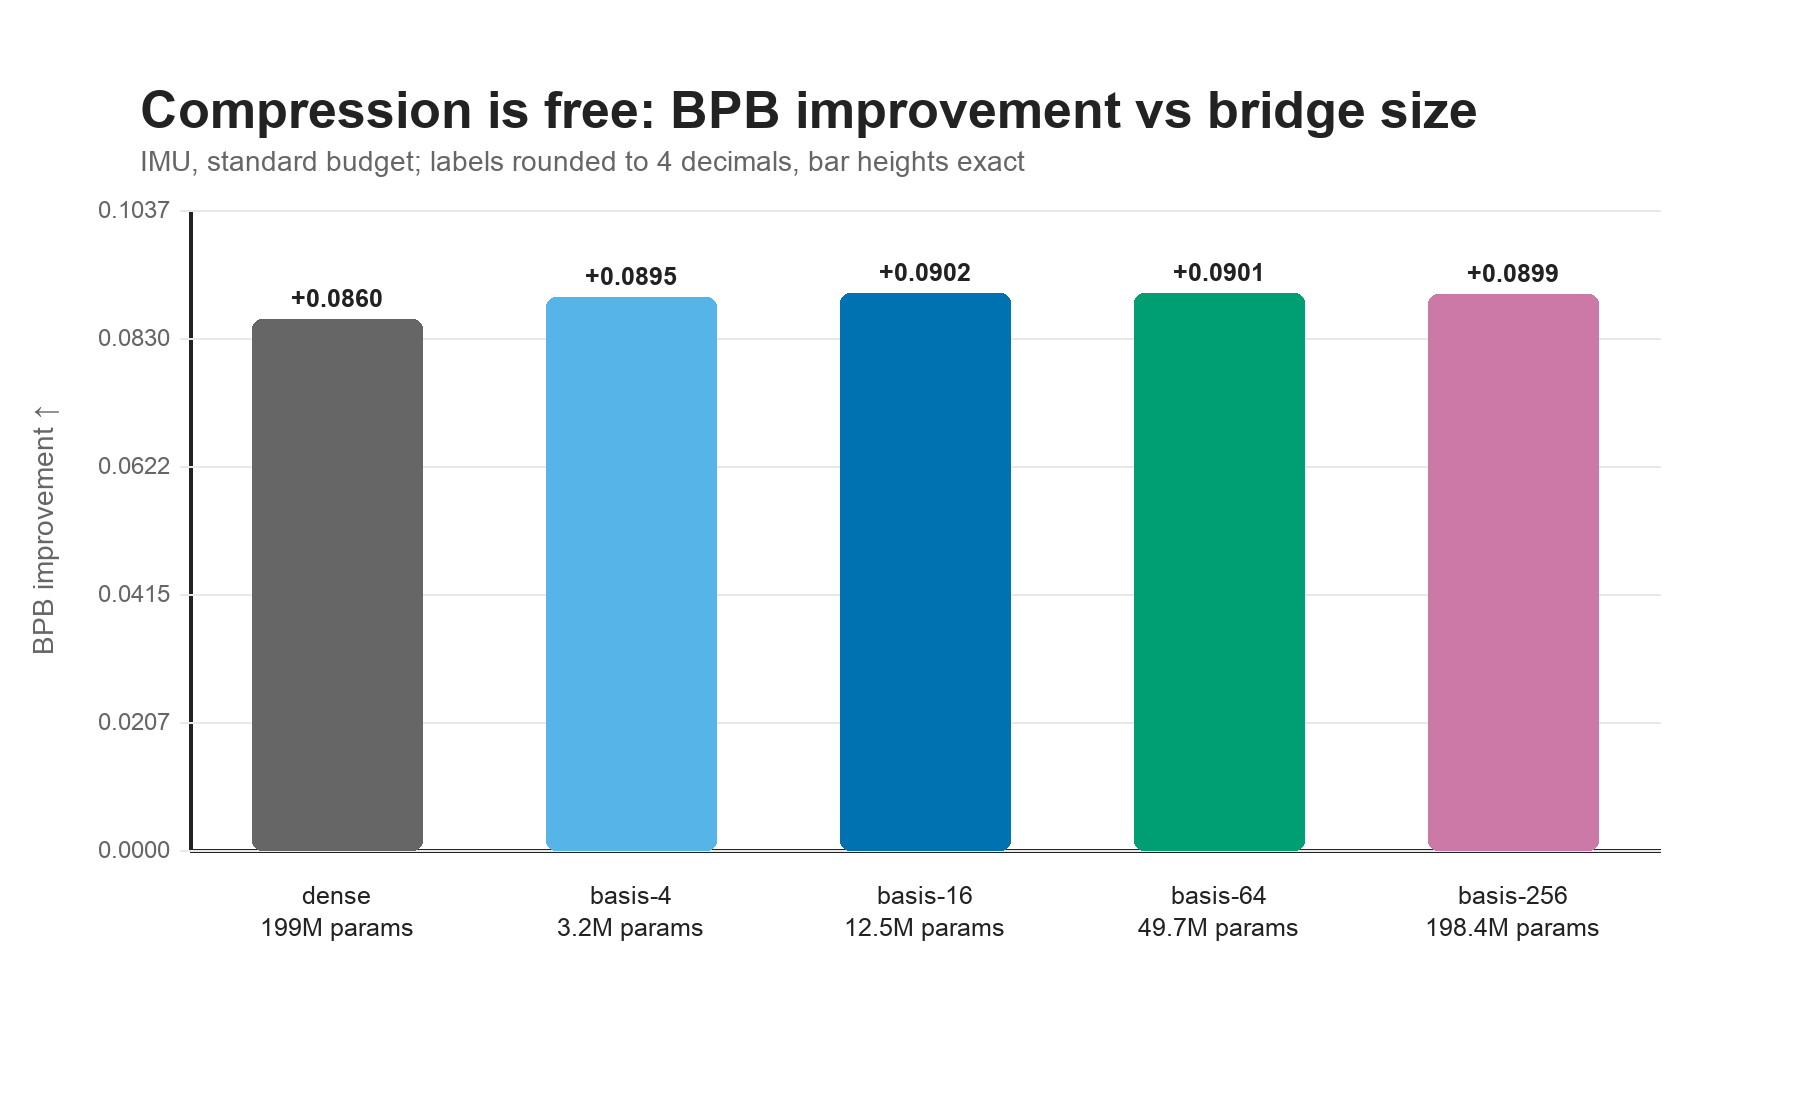
\includegraphics[width=0.82\linewidth]{paper2_capacity.png}
\caption{BPB improvement vs.\ bridge parameterization (IMU, standard budget). Every basis size matches or exceeds the dense bridge; labels round to four decimals while bar heights are exact.}
\label{fig:capacity}
\end{figure}

\subsection{Task conditioning: parity for trained bases}
Table~\ref{tab:imutask} reports the six-way IMU probe over five seeds per parameterization. The trained $k{=}16$ bridge averages 0.82 rank-1 against the dense bridge's 0.75; every control (no-bridge, shuffled, random features) sits at chance in every run. The seed spread is large enough to swallow that difference: dense runs from 0.65 to 0.83 (s.d.\ 0.071) and basis-16 from 0.67 to 0.91 (s.d.\ 0.106), so a 0.075 gap between five-seed means is not a difference we can claim. The honest reading is parity, now measured rather than asserted: reparameterizing to a 16-dimensional coefficient space costs nothing detectable on this task at 16$\times$ fewer parameters. Single-seed values for $k{=}64$ and $k{=}256$ fall inside the same spread. The fifty-way audio probe separates the parameterizations more sharply at the standard budget: trained bases reach 0.12 ($k{=}16$), 0.09 ($k{=}64$), and 0.14 ($k{=}256$) against the dense bridge's 0.31: well above chance, well below dense. Section~\ref{sec:span} shows this gap closing with training budget for $k{=}256$; we did not budget-extend the smaller $k$.

\begin{table}[t]
\centering
\caption{Six-way IMU task probe (rank-1 accuracy, chance 0.17), true-feature condition; all controls at chance in every run. Frozen rows use the basis at random initialization.}
\label{tab:imutask}
\begin{tabular}{lll}
\toprule
Bridge & Per-seed rank-1 & Mean \\
\midrule
dense (trained) & 0.72, 0.80, 0.83 & 0.78 \\
basis-16 (trained) & 0.91, 0.75, 0.67 & 0.78 \\
basis-64 (trained) & 0.58 & 0.58 \\
basis-256 (trained) & 0.75 & 0.75 \\
basis-16 (frozen) & 0.17 & 0.17 \\
basis-64 (frozen) & 0.59 & 0.59 \\
basis-256 (frozen) & 0.67 & 0.67 \\
\bottomrule
\end{tabular}
\end{table}

\subsection{The diversity--quality tradeoff dissolves in coefficient space}
For dense bridges, enforcing input-dependent weights costs language-modeling quality: at $\lambda = 0.10$ the dense bridge gives up 0.0086 BPB to reach cross-input cosine 0.60, and the original small-model study reported complete erasure at the strongest penalty. Table~\ref{tab:lambda} shows the trained $k{=}16$ bridge escaping the tradeoff entirely: cosine falls monotonically from 1.00 to 0.01, giving near-orthogonal per-input weights, while $\Delta$BPB stays within noise of its unregularized value (+0.0897 vs +0.0902). In a 16-dimensional coefficient space, input-dependence and text quality stop competing: the basis can orient its few directions so that both objectives are satisfiable at once. The frozen variant does not share this property (its diversity cost ratio resembles the dense bridge's), so free diversity is specifically a property of \emph{trained} low-dimensional coefficient spaces.

\begin{table}[t]
\centering
\caption{Diversity sweep on IMU (standard budget, seed 42): the dense bridge trades BPB for input-dependence; the trained basis-16 bridge does not.}
\label{tab:lambda}
\begin{tabular}{rrrrr}
\toprule
 & \multicolumn{2}{c}{dense} & \multicolumn{2}{c}{basis-16 (trained)} \\
$\lambda$ & $\Delta$BPB & Cross-cos & $\Delta$BPB & Cross-cos \\
\midrule
0.00 & +0.0860 & 0.99 & +0.0902 & 1.00 \\
0.05 & +0.0837 & 0.96 & +0.0890 & 0.02 \\
0.10 & +0.0774 & 0.60 & +0.0895 & 0.01 \\
0.20 & +0.0767 & 0.72 & +0.0897 & 0.01 \\
\bottomrule
\end{tabular}
\end{table}

\subsection{Span: a ramp, not a threshold}
\label{sec:span}
Table~\ref{tab:span} maps frozen-basis conditioning against $k$ at both task complexities. An earlier version of this study measured two points per task and reported a \emph{span threshold} bracketing them. With five widths per task the structure is visible, and it is not a threshold: conditioning rises monotonically and gradually with $k$. On the six-way IMU probe a frozen basis moves from chance at $k{=}16$ (0.17) through 0.27 at $k{=}32$ and 0.47 at $k{=}48$ to 0.62 at $k{=}96$, after which it flattens. Nothing in that sequence marks a boundary; a bracket drawn between any two adjacent points would have looked like a threshold.

What survives, and is now much better supported, is the complexity scaling. The two ramps are offset: at $k{=}48$ the IMU probe is already well clear of chance (0.47 against 0.17) while the fifty-way audio probe is still at it (0.032 against 0.02). Audio lifts first at $k{=}96$ (0.063) and reaches 0.19 by $k{=}256$. A random subspace has to be wider for the harder task, which is the intrinsic-dimension picture applied to a generated update: training inside a random subspace works once the subspace is wide enough to intersect the solution set, and the required width is a property of the task \cite{li2018intrinsic,aghajanyan2021intrinsic}. What differs here is that the subspace carries a \emph{per-input} family of updates rather than one fixed adaptation, so the width is set by the family the task demands.

The practical consequence is milder than a threshold rule and easier to apply. There is no width at which a frozen basis switches on, so sizing $k$ is a cost curve rather than a boundary: pick the smallest width whose conditioning is good enough for the deployment, and expect diminishing returns rather than a cliff. The $k{=}16$ frozen bridge remains a genuine floor, though, with the IMU probe at chance and the capacity gain gone under regularization ($\Delta$BPB +0.0001): sixteen random directions in a 774,144-dimensional weight space span nothing useful, and at that width the basis must be learned.

\begin{table}[t]
\centering
\caption{Frozen-basis task conditioning against basis width $k$ (rank-1 accuracy, true-feature condition; IMU chance 0.17 at 600 steps, audio chance 0.02 at 1200 steps). Cells give the seed mean with $n$ where more than one seed was run; $k{=}16$, 64, and 256 are the original single-seed points. Both columns rise monotonically, and the audio ramp arrives later than the IMU one.}
\label{tab:span}
\begin{tabular}{rll}
\toprule
$k$ & IMU (six-way) & Audio (fifty-way) \\
\midrule
16 & 0.17 & -- \\
32 & 0.27 {\footnotesize ($n{=}3$)} & 0.03 {\footnotesize ($n{=}3$)} \\
48 & 0.47 {\footnotesize ($n{=}3$)} & 0.03 {\footnotesize ($n{=}3$)} \\
64 & 0.59 & 0.03 \\
96 & 0.62 {\footnotesize ($n{=}3$)} & 0.06 {\footnotesize ($n{=}3$)} \\
128 & 0.64 {\footnotesize ($n{=}3$)} & 0.07 {\footnotesize ($n{=}3$)} \\
256 & 0.67 & 0.19 \\
\bottomrule
\end{tabular}
\end{table}

High on the ramp, freezing is an advantage rather than a compromise. Table~\ref{tab:budget} and Figure~\ref{fig:budget} track the fifty-way audio probe across training budgets: the frozen $k{=}256$ bridge reaches 0.36 mean rank-1 at 2400 steps (three seeds), the level the dense bridge reaches at 1200 (0.33). That is dense-level conditioning at $\sim$$2\times$ the steps from 0.09\% of the trainable parameters, with the basis reproducible from a seed rather than stored. The same table shows the trained $k{=}256$ basis \emph{trailing} its own frozen variant at 2400 steps (0.28 vs 0.36): high on the ramp, a churning basis is a moving target for the coefficient head, and stationarity wins. The dense bridge continues to improve with budget (0.44 at 2400; 0.61 at 6000 in the replication note's $10\times$ suite \cite{penov2026note}), so the frozen regime buys its parameter economy with training compute, not with a performance ceiling we could detect.

\begin{table}[t]
\centering
\caption{Fifty-way audio task probe (rank-1, chance 0.02) vs.\ training budget, seed 42 except where noted. The frozen $k{=}256$ value at 2400 steps is a three-seed mean (per-seed values in parentheses).}
\label{tab:budget}
\begin{tabular}{rlll}
\toprule
Steps & dense & basis-256 (trained) & basis-256 (frozen) \\
\midrule
600 & 0.31 & 0.14 & -- \\
1200 & 0.33 & 0.20 & 0.19 \\
2400 & 0.44 & 0.28 & 0.36 (0.33, 0.41, 0.34) \\
\bottomrule
\end{tabular}
\end{table}


\begin{figure}[t]
\centering
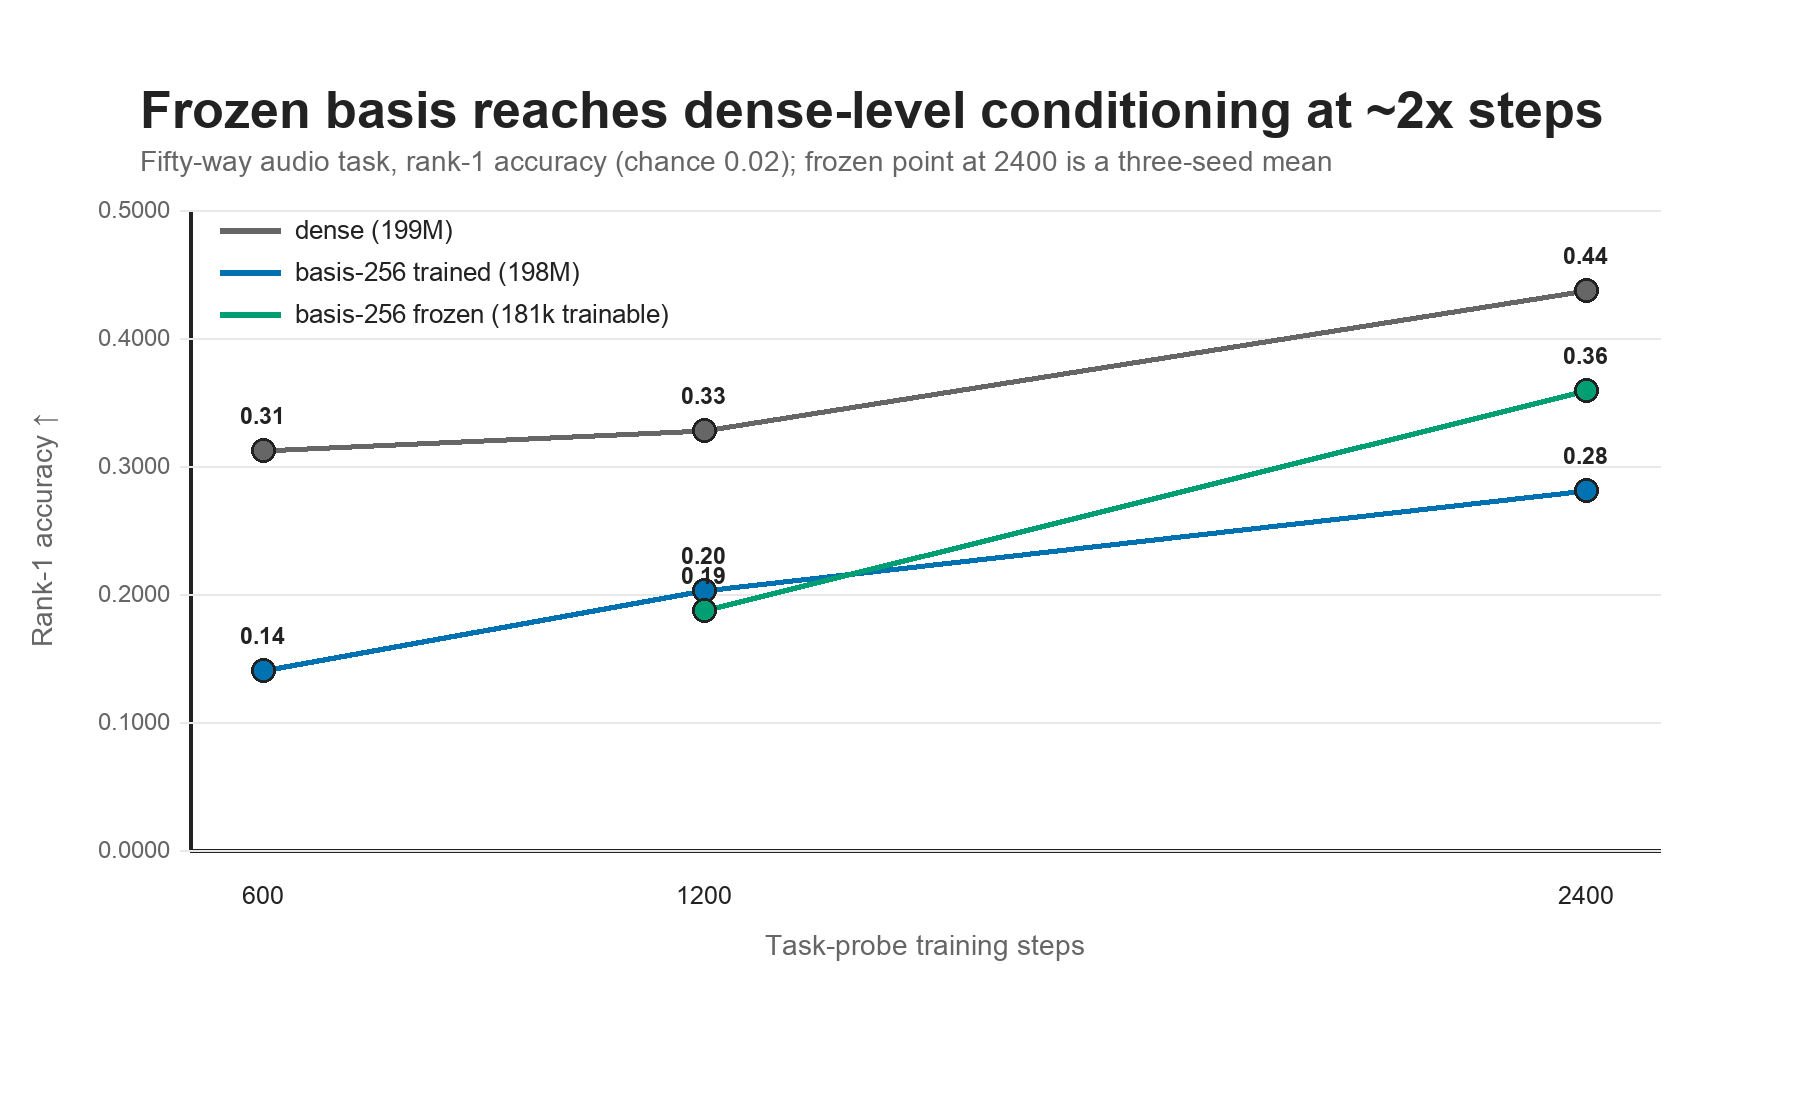
\includegraphics[width=0.82\linewidth]{paper2_audio_budget.png}
\caption{Fifty-way audio conditioning vs.\ training budget. The frozen $k{=}256$ bridge (181k trainable parameters) reaches at 2400 steps the level the dense bridge (199M) reaches at 1200; the trained basis trails its own frozen variant.}
\label{fig:budget}
\end{figure}

\subsection{What does not work}
\label{sec:negative}
\paragraph{Accelerating the basis.}
If the frozen regime's $2\times$ step cost came from a slowly-rotating basis, raising the basis learning rate should recover it. The opposite happens: at 1200 audio steps, scaling the basis learning rate by $3\times$ drops rank-1 from 0.20 to 0.06, and $10\times$ to 0.03, near chance. The coefficient head learns against the basis; making the basis move faster destroys the target it is learning to address. Consistent with this, the frozen basis at the same budget matches the trained one (0.19 vs 0.20): basis training contributes nothing at large $k$, and the head does all the work.

\paragraph{Composition by coefficient averaging.}
With a shared basis, averaging generated weights is algebraically identical to averaging coefficients ($\mathrm{mean}(c_i B) = \mathrm{mean}(c_i) B$), so the harness's additive-merge composition directly tests coefficient-space composition. Table~\ref{tab:compose}: it inherits the dense bridge's sub-additivity, slightly worse. The interference comes from the averaging operation, which dilutes each constituent's contribution regardless of the space it is expressed in. (The frozen row's low absolute values reflect its $2\times$ budget law: the 150-step bricks are under-trained, so its retention should be read with caution.) Constructive composition needs a different merge, not a different representation; we return to this in the discussion.

\begin{table}[t]
\centering
\caption{Additive-merge composition (BPB improvement; vision+audio+IMU triple vs.\ mean of singles; 150 steps/brick, standard protocol).}
\label{tab:compose}
\begin{tabular}{lrrr}
\toprule
Bridge & Singles mean & Triple & Retention \\
\midrule
dense & +0.0862 & +0.0636 & 74\% \\
basis-16 (trained) & +0.0866 & +0.0582 & 67\% \\
basis-256 (frozen) & +0.0420 & +0.0256 & 61\% \\
\bottomrule
\end{tabular}
\end{table}

\section{Related Work}
Training within a random low-dimensional subspace has a long precedent: Li et al.\ \cite{li2018intrinsic} measure the intrinsic dimension of an objective landscape by the smallest random subspace in which training still succeeds, and Aghajanyan et al.\ \cite{aghajanyan2021intrinsic} show that language-model fine-tuning has a low intrinsic dimension that shrinks with pretraining. Our span threshold is the same quantity measured for a per-input generated update rather than a single fixed one. Static-coefficient random-basis adaptation is well established: PRANC \cite{nooralinejad2023pranc} trains coefficients over seed-reconstructible pseudo-random basis networks; NOLA \cite{koohpayegani2024nola} applies the idea to LoRA factors; VeRA \cite{kopiczko2024vera} shares one frozen random matrix pair across layers with trained per-layer scalings; RandLoRA \cite{albert2025randlora} scales many frozen random low-rank matrices to full-rank updates; VB-LoRA \cite{li2024vblora} mixes from a shared \emph{learned} vector bank. All train coefficients once per task. Input-conditioned mixing exists over \emph{trained} factors: TopLoRA \cite{li2025toplora} generates per-token diagonal coefficients modulating learned per-module LoRA factors --- the closest prior work to ours --- HydraLoRA \cite{tian2024hydralora} routes per sample over trained expert heads, and the mixture-of-LoRA-experts line routes per token \cite{wu2024mole}. Hypernetworks that generate adapters condition on task descriptions or exemplars rather than individual inputs: HyperTuning \cite{phang2022hypertuning}, Text-to-LoRA \cite{charakorn2025texttolora}. Against all three lines, our setting combines a frozen \emph{random} shared basis with coefficients generated \emph{per input} by a hypernetwork --- and conditioned on an external sensor stream rather than the text itself \cite{penov2026bridges}. To our knowledge no prior work occupies this intersection, and none reports an analog of the span threshold, the free-diversity property of trained low-dimensional coefficient spaces, or capacity-vs-conditioning probes for generated weights. LoRA composition via learned per-task mixing (LoraHub \cite{huang2024lorahub}) contrasts with our per-input merge negative; tying and factor-freezing for parameter economy appear in Tied-LoRA \cite{renduchintala2024tiedlora} and LoRA-XS \cite{balazy2024loraxs}.

\section{Discussion}
The two regimes answer different engineering questions. When bridge quality and conditioning fidelity dominate (a deployed always-on sensor with a modest parameter budget), the trained small basis dominates the dense bridge on the axes we measured for single-sensor deployment: 16$\times$ smaller, language-modeling gain slightly higher, six-way conditioning at parity, and diversity regularization free. It still shares the family's step-for-parameter trade on harder tasks and, like every parameterization tested, composes sub-additively. When parameter and storage economy dominate (many sensors, many model versions, over-the-air updates), the frozen seeded basis reduces the entire sensor-specific artifact to a $\sim$181k-parameter head plus a seed, at the cost of a task-complexity-dependent minimum $k$ and roughly doubled training. The span ramp gives the selection rule, and its gradualness makes that rule forgiving: there is no width to clear, so size $k$ by the conditioning the deployment needs and expect diminishing returns rather than a cliff. Train the basis only at the smallest widths, where a random subspace spans nothing.

The composition negative sharpens the agenda the original paper left open. Since the interference comes from the merge operation rather than the representation, the shared frozen basis becomes an asset rather than a fix: it makes \emph{disjoint coefficient allocation} trivial (each modality claims its own block of an orthonormal basis, making weight-space interference zero by construction), and it makes task-level composition probes the right instrument, since BPB retention mostly measures adaptation magnitude surviving a mean. Both are mechanical extensions of the present harness.

\section{Limitations}
All results are on one pretrained base model and two sensor task complexities. The span ramp is mapped at five widths per task with three seeds at the four new widths, but the three original widths ($k{=}16$, 64, 256) remain single-seed, and the IMU ramp is noisy enough at small $k$ that individual points should not be over-read. The $\lambda$ sweep is still single-seed; the IMU probe's own seed spread is wide, so per-$k$ differences on the easy task should not be over-read. The frozen regime's $2\times$ step law is measured at one task and bracketed budgets. BPB retention is a weak composition metric, used here only to show the negative transfers across parameterizations. Conclusions about scale inherit the caveats of the replication note \cite{penov2026note}, including the pretraining-vs-scale confound.

\section{Conclusion}
Reparameterizing a conditional LoRA bridge's output as coefficients over a basis of LoRA directions turns its main scaling liability into a design space with two useful regimes: a trained low-dimensional regime that compresses 16$\times$ while dissolving the diversity--quality tradeoff, and a frozen seeded regime that reduces the trainable and storable footprint to a coefficient head at 0.09\% of the dense bridge, for a measured $2\times$ training cost. A span ramp whose position grows with task complexity separates the regimes and gives practitioners a selection rule; mapping it at five widths per task showed the boundary we first reported to be a gradual rise rather than a threshold. The failures are as instructive as the successes: the basis should be stationary or absent, not fast, and composition fails in coefficient space exactly as it does in weight space. That locates the problem in the merge operation, and makes disjoint allocation over a shared frozen basis the next constructive step.

\section*{Reproducibility Statement}
All experiments run through the published bridge harness with the basis parameterization selected by \texttt{--bridge basis-<k>} and the frozen variant by \texttt{--basis-lr-scale 0}. Every number in this manuscript is rendered from three bundled artifacts (the basis-sweep summary and the two dense reference suites) by the repository's renderer; run names in the sweep artifact encode each experiment's configuration. Code, artifacts, and the exact render pipeline: \url{https://github.com/kortexa-ai/legolm.basis}.

\bibliographystyle{plain}
\bibliography{references}
\end{document}
